\documentclass[12pt]{article}

\usepackage{sbc-template}

\usepackage{graphicx,url}

\usepackage[brazil]{babel}   
%\usepackage[latin1]{inputenc}  
\usepackage[utf8]{inputenc}  
% UTF-8 encoding is recommended by ShareLaTex

     
\sloppy

\title{Fundamentals of Digital Entrepreneurship}

\author{Danilo Fiorotto\inst{1}, Linn Holm\inst{1}, Matheus Redecker\inst{1} }


\address{Pontifícia Universidade Católica do Rio Grande do Sul
 \email{\{matheus.redecker, linn.holm, danilo.fiorotto\}@acad.pucrs.br}
}

\begin{document} 

\maketitle

\section{Introduction}
This paper is to show how the Fundamentals of Digital Entrepreneurship class given by Rafael Channin guide us to pass thought all the process of begin a undertaking since the idea until the project in work. In the next sections we will explain the whole process, begin with the idea in a brainstorm, follow by the construction of the canvas, after this make the experiments and a section about what we have learn about all the process.

\section{The idea}
In our group we have a exchange student from Switzerland and when we are discussing about ideas she tell us about the things that we want here that already exist there and with one of this things we decide to make our project about it. The on-line supermarket, the main idea is buy the same things that you can buy in a physic supermarket but do it at home. Our thinking was that we may save time and help how have problems in reach to the supermarket. This hypothesis were tested and showed in the following sections.

\section{Lean Canvas}

Lean Canvas was created by Ash Maurya. It came to oppose the Business plan. As it says in leanStack\footnote{http://leanstack.com/lean-canvas/} website: "Business plans take too long to write, are seldom updated, and almost never read by others but documenting your hypotheses is key. Lean Canvas solves this problem using a 1-page business model that takes under 20 minutes to create.". The propose of Lean Canvas is to build something fast and start testing your assumptions, if you fail it need to be fast for you learn with the process and start again with a different approach. \\
After we decided to try to establish a idea of a on line supermarket here in 
Brazil, following the example in Sweden, we started working on our Lean 
Canvas, for inexperience administrative students, Lean Canvas helped us a
lot, because Lean Canvas is simple, easy and fast to use and understand, 
and also we are trying to build a new business model here in Brazil, or at least in Porto Alegre, so Lean Canvas helped aus in a point that we can just stick some notes and if is not good we could change everything  and stick other things.We build our lean canvas starting with “what problem do we solve?” So we decide some possible problems to start.After we decide to reach the main problem that is “Time” we start think about our solution and our unique value proposition and also our key metrics. But the hardest thing was think about customers segments, but just customers, but how to “filter” and reach the exactly customer that will buy our product/service. After a lot of discussion we decide to work with full time workers, families and students ( problem of students is not time, but could be transportation). Done that, channels was our concern, but was not a big problem, we choose to keep using on line channels. The financial part of our lean canvas, was not so specified because we decide to focus in what we gonna need to pay/spend Money, and at this point the exactly value is not the problem for us. Finishing with our Revenue, we decided how to retain customers and how to have profit with our customers, finalizing with two main customers 
(Subscribers and Spontaneous).\\
Once the canvas is done we are able to go out and test our idea and as said before as soon as you test ass soon as you can fail and choose a different direction to your idea. Our canvas filled can be viewed below: 

\begin{figure}[ht]
\centering
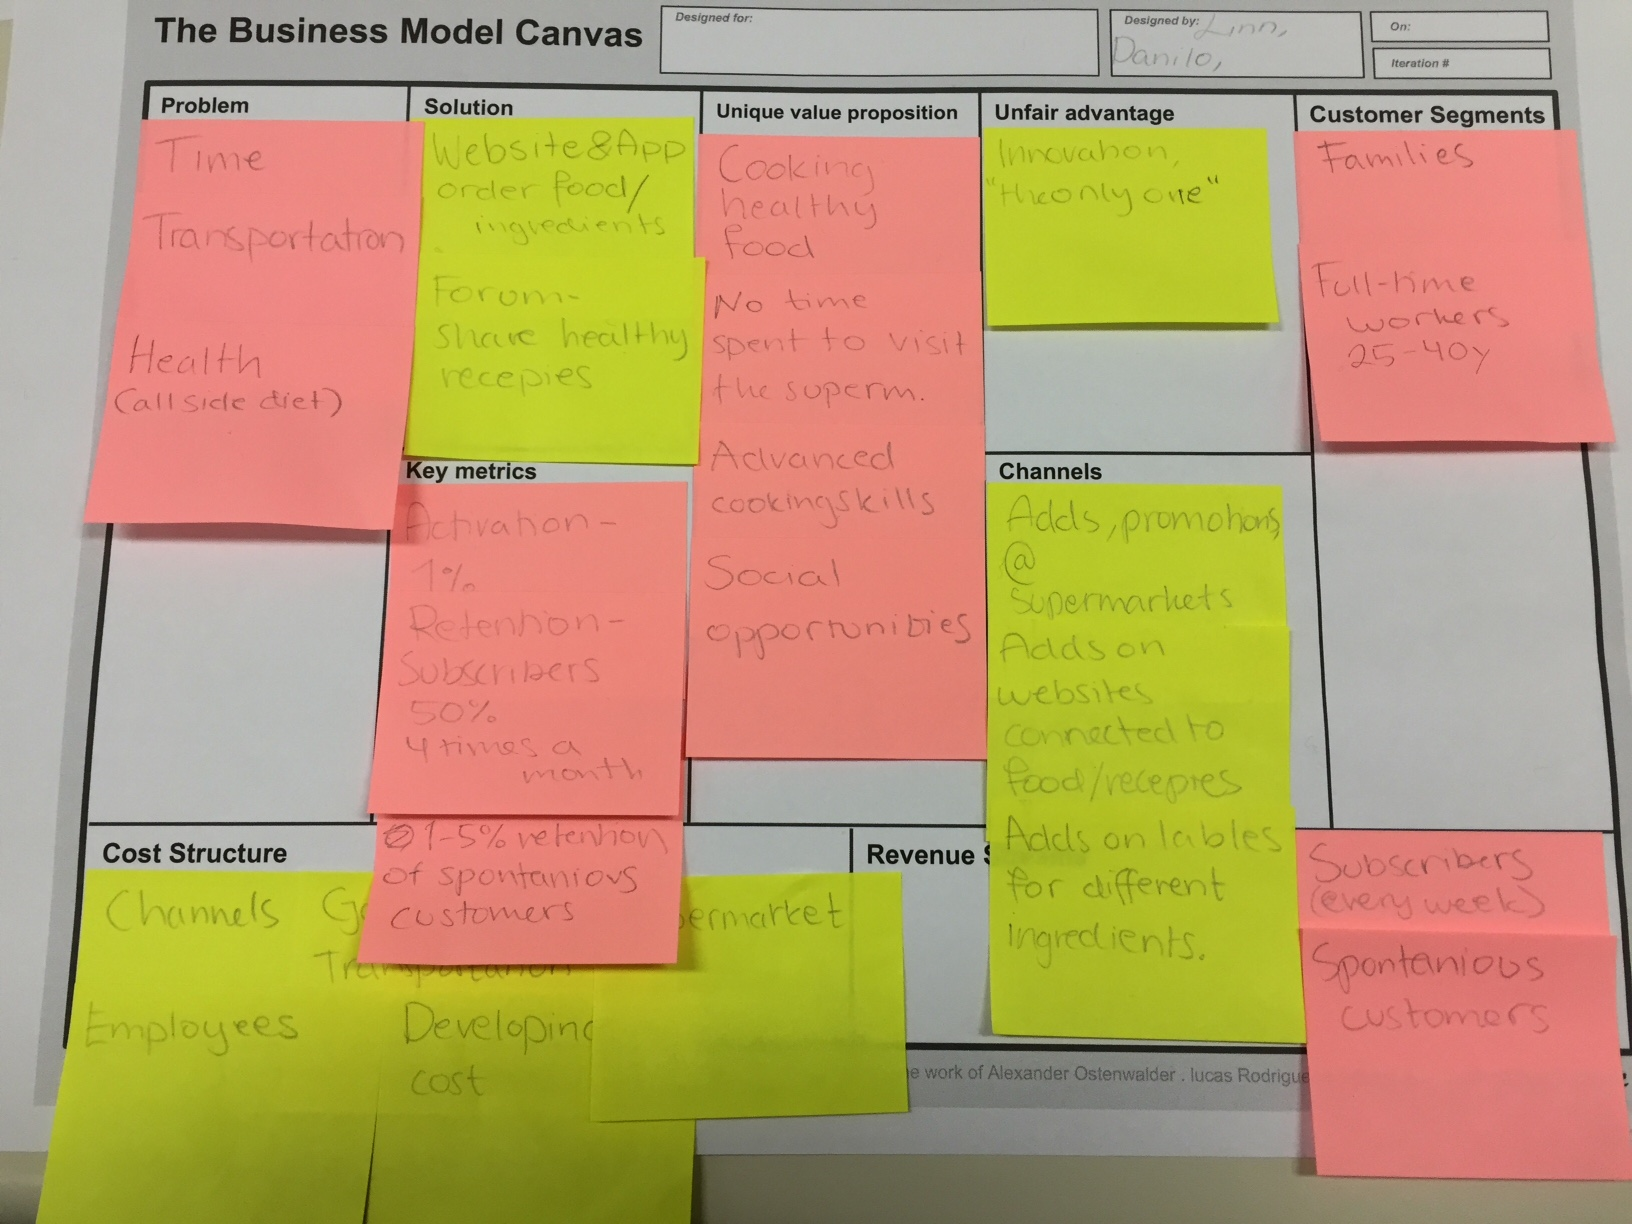
\includegraphics[scale=0.25]{IMG_0311.JPG}
\label{first-canvas}
\end{figure}

\section{Experiments}

All the ideas is in our lean canvas and we need to test, after learning about 
Customer Development Process we start working filling the Javelin Board. 
Filling our Javelin, we discuss about some numbers, like our success criteria 
and, what is the main problem that we need to test at the first time, and 
how we gonna interview people.
Done that we went outside the room, and start interviewing people, we 
started with full time workers around PUCRS, we interview some lab 
technicians, administrative workers from some officers, professors and some 
interns/students that are walking around, a lot of people, don’t like to talk in 
the first time, but after we ask somethings, people get comfortable and talk 
normally with us.
When we return to class we put everything on paper and count how many 
people have problems going to supermarket, how many people like to go, 
or people that dislike that.
And analyzing everything we saw that time, maybe is not our problem, and 
maybe people like go to supermarket.
So we run again the experiment but now if students and looking for another
type of problem, and we again fail in our success criteria. At the last time we 
try something different, we decide to ask different questions, like: “what you 
think about an on line supermarket”, “you will feel comfortable if you do not
need to go to supermarket again?”
And also we ask for an email if they interested in our idea and for our 
surprise we got 5 emails in 5 interviews.
That means that our main points could be wrong and if you do not spend 
time doing your customers development, you maybe will fail in your Project. \\
In the first moment we assume that people do not like to go to the supermarket and our idea was to free the people of this job. But when we did the first experiment with full time workers and try to solve the time problem. We discover that people enjoy go to the supermarket and see what they are buying, we had some disappointment with this learning, then in the second experiment we tried a different experiment to test the students with problems about transportation and again we fail in reach the real problem, but in this two experiments we did not talked about the product and learn about the potential customers some interesting things, they think people in the supermarket not polite even the employers, they do not like the waiting. In our final experiment we can tell the people about the product just not try to pitch the idea, let them talk what they really think, and the result is amazing, we interviewed some of the people that answered in the first and the second experiment, the same people how do not had the problem, and they like the idea and gave contact for us. We conclude with this that people do not know they have the problem until we show them. The next step is to put the project ahead and start to talk with the supermarkets if they want to make some partner and if this reply be positive begin the development phase and after it advertise for the right costumers.\\
The tests detailed above you can see filled in the Javelin Board below: 

\begin{figure}[ht]
\centering
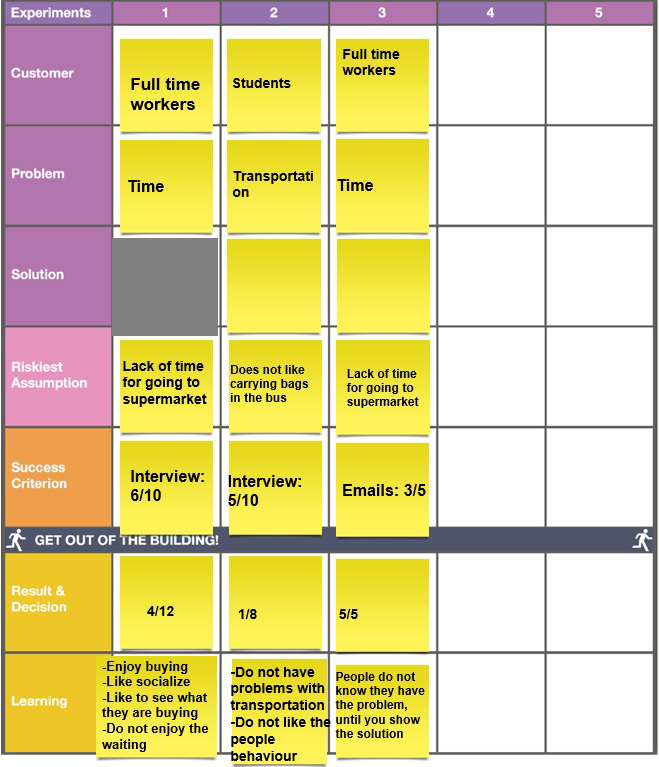
\includegraphics[scale=0.5]{experiments.jpg}
\end{figure}

\section{Conclusion}
The project make us see that begin a undertaking is not easy but also is not impossible. We begin with an idea that change when we start to talk with the potentials costumers, we discover things that never pass thought our heads, for example, people enjoy go to the supermarket, just because we do not like it does not mean that everyone are the same. \\
The entire process help to make a good way to discover what the next step with the project, fast, easy and cheap, what all the startups need. You can pivot you idea as soon as you see that have a better or a different way to do what you are intend to do. Fail fast is a great lesson that we can carry for life.       



\end{document}
